%begmin%
	\begin{minipage}{0.47\textwidth}
		\item Una llave de agua suministra un caudal constante $Q_a$ a un tubo capilar vertical de área $A$. El agua fluye a través del tubo capilar por una tubería cilíndrica horizontal de radio $R$ y largo $L$, como se muestra en la figura. El caudal $Q_c$ que sale por el capilar y el perfil de velocidades $v(r)$ está dado por la Ley de Poiseuille como:
		\begin{equation*}
			Q_c = \dfrac{\pi \Delta p R^4}{8 \eta L} \hspace{10mm} v(r) = \dfrac{\Delta p}{4 \eta L} \left( R^2 - r^2\right)
		\end{equation*}
		\noindent donde la viscosidad del fluido es $\eta$.
	\end{minipage}
	\begin{minipage}{0.5\textwidth}
		\begin{center}
			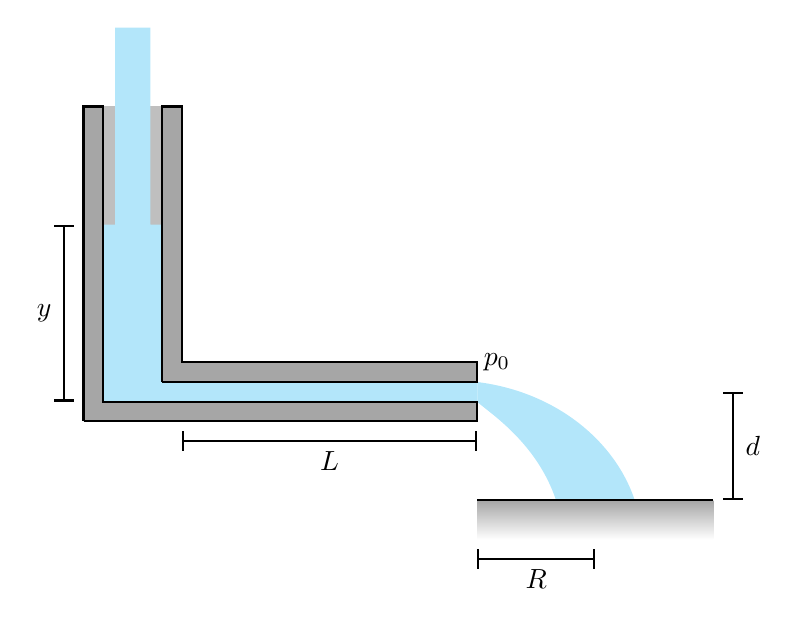
\begin{tikzpicture}[scale=.5]
			%alcance%
			\fill [fill=white!50!gray] (0,5)rectangle(2.5,8);
			\fill [fill=cyan!30!white] (0,0)--(10,0)--(10,1.5)--(2.5,1.5)--(2.5,5)--(0,5)--(0,0)
			(.8,5)rectangle(1.7,10);
			\fill [fill=cyan!30!white] (10,1) ..controls (12,.75) and (13.5,-.5).. (14,-2)--(12,-2) .. controls (11.5,-.5) and (10.25,.25) .. (10,.5);
			\filldraw [fill=white!30!gray,thick] (0,0)--(10,0)--(10,.5)--(.5,.5)--(.5,8)--(0,8)--(0,0) 
			(2,1)--(10,1)--(10,1.5)--(2.5,1.5)--(2.5,8)--(2,8)--(2,1);
			\shade [top color=white!30!gray,bottom color=white] (10,-2)rectangle(16,-3);
			\draw [thick] (10,-2)--(16,-2); 
			\draw [thick, |-|] (2.5,-.5)--(10,-.5);
			\draw [thick, |-|] (-.5,.5)--(-.5,5);
			\draw [thick, |-|] (16.5,-2)--(16.5,.75);
			\draw [thick, |-|] (10,-3.5)--(13,-3.5);
			\draw [dotted]
			(-1,2.75) node[scale=1] {\(y\)}
			(6.25,-1) node[scale=1] {\(L\)}
			(11.5,-4) node[scale=1] {\(R\)}
			(17,-.625) node[scale=1] {\(d\)}
			(10.5,1.5) node[scale=1] {\(p_0\)}
			;
			\end{tikzpicture}
		\end{center}
	\end{minipage}
%endmin%

\begin{enumerate}[a)]
	\item Determine la altura máxima en el capilar.
	\item Determine el máximo alcance horizontal $R$ que sale por el capilar para una altura $d$.
	\item Determine el tiempo $t$ en función de la altura $y$, considere que para $t=0$ el capilar está vacío.
\end{enumerate}

\underline{\textbf{Solución:}}

\begin{enumerate}[a)]
	
	\item  La altura máxima dentro del tubo vertical (\(y_{\text{max}}\)) se alcanza cuando el caudal de entrada es igual al de salida (\( Q_a = Q_c \)). Observe que siempre \( Q_c \leq Q_a \):
	
	\begin{equation*}
		Q_a = \frac{\pi \Delta p R^4}{8 \eta L}
	\end{equation*}
	
	donde: 
	
	\begin{align*}
		\Delta p &= \cancel{p_0} + \rho g y_{\text{max}} - \cancel{p_0} \\
		\Delta p &= \rho g y_{\text{max}}\\
		\Rightarrow Q_a &= \frac{\pi \rho g y_{\text{max} R^4} }{8 \eta L}
	\end{align*}
	
	Entonces la altura máxima del capilar es igual a:
	\begin{equation}
	\tcbhighmath{y_{\text{max}} = \dfrac{8 Q_a \eta L}{\pi \rho g R^4}}
	\end{equation}
	
	\item La máxima velocidad de salida se obtiene para el centro de la tubería, $v(r=0)=v_{\text{max}}$, cuya expresión es:
	\begin{align*}
	v_{\text{max}} &= \frac{\Delta p}{4 \eta L}R^2 \\
	v_{\text{max}} (y) &= \frac{\rho g y}{4 \eta L}R^2
	\end{align*}
	
	Luego, la velocidad máxima de \(v_{\text{max}}(y)\) se obtiene para \(y_{\text{max}}\):
	\begin{equation*}
	v_{\text{max}} = v_{\text{max}}\left(y_{\text{max}}\right)
	\end{equation*}
	
	Por otro lado, el tiempo de vuelo $t_v$ (tiempo en que se mantiene en el aire el fluido que sale por la tubería horizontal), está dado por:
	\begin{align*}
		d &= \frac{1}{2} g t_{\text{v}}^2 \\
		\Rightarrow t_{\text{v}} &= \sqrt{\frac{2d}{g}}
	\end{align*}
	
	Como la componente horizontal de velocidad del flujo del agua a la salida no varía en el tiempo, se tiene que \( R_{\text{max}} \)
	
	\begin{align*}
	R_{\text{max}} &= v_{\text{max}} \ t_{\text{v}}\\
	&= \frac{\rho g y_{\text{max}}}{4 \eta L} \ R^2\sqrt{\frac{2d}{g}}
	\end{align*}
	
	Entonces \(R_{\text{max}}\) es igual a:
	
	\begin{equation*}
	\tcbhighmath{ R_{\text{max}} = \dfrac{\rho \ y_{\text{max}} R^2}{4\eta L} \ \sqrt{2dg} = \dfrac{2 Q_a}{\pi R^2} \sqrt{\dfrac{2d}{g}}} 
	\end{equation*}
	
	
	\item Se tiene que el balance de masa dentro de la tubería está dado por:
	
	\begin{equation*}
		\frac{dV}{dt} = Q_a - Q_c
	\end{equation*}
	
	donde 
	\begin{align*}
	V &= A \ y(t) \\
	\frac{dV}{dt} &= A \ \frac{dy}{dt}\\
	\Rightarrow A \ \frac{dy}{dt} &= Q_a - \frac{\pi \rho g y R^4}{8 \eta L}
	\end{align*}
	
	Utilizando \(\beta = \frac{\pi \rho g R^4}{8 \eta L}\)
	
	\begin{align*}
	A \ \frac{dy}{dt} &= Q_a - \beta y\\
	\Rightarrow dt &= A \ \frac{dy}{Q_a - \beta y} \\
	\int_{0}^{t} dt &= A\int_{0}^{y} \frac{dy}{Q_a - \beta y}\\
	\Rightarrow t &= \frac{A}{\beta} \ \ln\left( \frac{Q_a}{Q_a-\beta y} \right)
	\end{align*}
	
	Reemplazando \(\beta\) se tiene que el tiempo \(t\) equivale a:
	\begin{equation*}
	\tcbhighmath{t = \dfrac{8 A \eta L}{\pi \rho g R^4} \ \ln \left( \frac{Q_a}{Q_a - \frac{\pi \rho g R^4}{8\eta L}y} \right)}
	\end{equation*}
	
\end{enumerate}
